\documentclass[12pt]{article}

\usepackage{times}
\usepackage{graphicx}
\usepackage{amsmath}
\usepackage{url}

\setlength{\textwidth}{6.5in}
\setlength{\textheight}{8.9in}
\setlength{\oddsidemargin}{0.0in}
\setlength{\topmargin}{0.05in}
\setlength{\headheight}{-0.05in}
\setlength{\headsep}{0.0in}

\newcommand{\indep}{\perp\!\!\!\perp}

\begin{document}

\begin{center}
{\bf CS 6300} \hfill {\large\bf HW07: Bayes Nets I \hfill April 4, 2023}
\end{center}

\section{D-Separation}

For the Bayes net below, determine if each independence assertion is guaranteed to be true.

\begin{center}
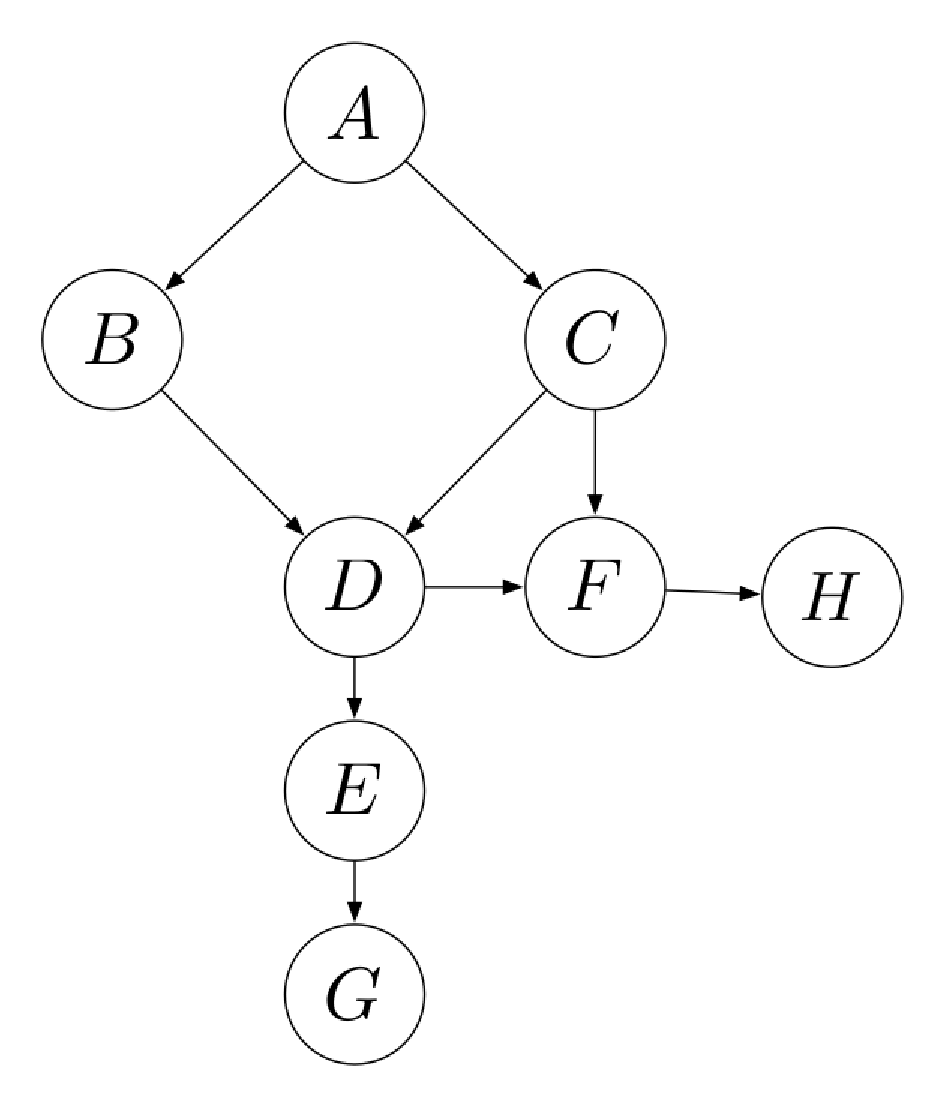
\includegraphics[width=0.35\linewidth]{bayes.eps}
\end{center}
    
\begin{enumerate}

\item $B \indep C$ 

Paths: BAC, BDC, and BDFC

Triples: \\
BAC - Active \\
BDC - \\
BDF - \\
DFC - 

Any active path indicates not guaranteed. BAC is active

\item $B \indep C \mid G$ 

Paths: BAC, BDC, and BDFC

Triples: \\
BAC - Active \\
BDC - \\
BDF - \\
DFC - 

Any active path indicates not guaranteed. BAC is active

\item $B \indep C \mid H$ 

Paths: BAC, BDC, and BDFC

Triples: \\
BAC - Active \\
BDC - \\
BDF - \\
DFC - 

Any active path indicates not guaranteed. BAC is active

\item $A \indep D \mid G$ 

Paths: ABD, ACD, and ACFD

Triples: \\
ABD - Active \\
ACD - \\
ACF -  \\
CFD - 

Any active path indicates not guaranteed. ABD is active

\item $A \indep D \mid H$

Paths: ABD, ACD, and ACFD

Triples: \\
ABD - Active \\
ACD - \\
ACF -  \\
CFD - 

Any active path indicates not guaranteed. ABD is active

\item $B \indep C \mid A, F$ 

Paths: BAC, BDC, and BDFC

Triples: \\
BAC - Inactive \\
BDC - Inactive \\
BDF - Active \\
DFC - Active

Any active path indicates not guaranteed. BDFC is active

\item $F \indep B \mid D, A$

Paths: FDB, FCAB, FCDB, and FDCAB

Triples: \\
FDB - Inactive \\
FCA - \\
CAB - Inactive \\
FCD - Active\\
CDB - Active\\
FDC - Inactive\\
DCA - 

Any active path indicates not guaranteed. FCDB is active.

\item $F \indep B \mid D, C$ 

Paths: FDB, FCAB, FCDB, and FDCAB

Triples: \\
FDB - Inactive\\
FCA - Inactive\\
CAB - \\
FCD - Inactive\\
CDB - \\
FDC - Inactive \\
DCA - 

All paths are have an inactive triple and are thus inactive, therefore we are guaranteed that the independence assertion is true

\end{enumerate}

% cs 188 sp11 final.

\clearpage

\section{Inference by Enumeration}

Consider the following Bayes' net.  Derive $P(A|+e,-f)$.

\begin{tabular}{cc}
\begin{tabular}{cc}
\begin{tabular}{|r|r|} \hline
A  & $P(A)$ \\ \hline
+a & 0.3      \\ \hline
-a & 0.7      \\ \hline
\end{tabular} &
\begin{tabular}{|r|r|r|} \hline
B  & A  & $P(B|A)$ \\ \hline
+b & +a & 0.7      \\ \hline
+b & -a & 0.6      \\ \hline
\end{tabular} \\[.5in]
\begin{tabular}{|r|r|r|} \hline
C  & A  & $P(C|A)$ \\ \hline
+c & +a & 0.2      \\ \hline
+c & -a & 0.9      \\ \hline
\end{tabular} &
\begin{tabular}{|r|r|r|} \hline
D  & B  & $P(D|B)$ \\ \hline
+d & +b & 0.3      \\ \hline
+d & -b & 0.4      \\ \hline
\end{tabular} \\[.5in]
\begin{tabular}{|r|r|r|} \hline
E  & C  & $P(E|C)$ \\ \hline
+e & +c & 0.4      \\ \hline
+e & -c & 0.5      \\ \hline
\end{tabular} &
\begin{tabular}{|r|r|r|} \hline
F  & C  & $P(F|C)$ \\ \hline
+f & +c & 0.1      \\ \hline
+f & -c & 0.8      \\ \hline
\end{tabular}
\end{tabular} & 
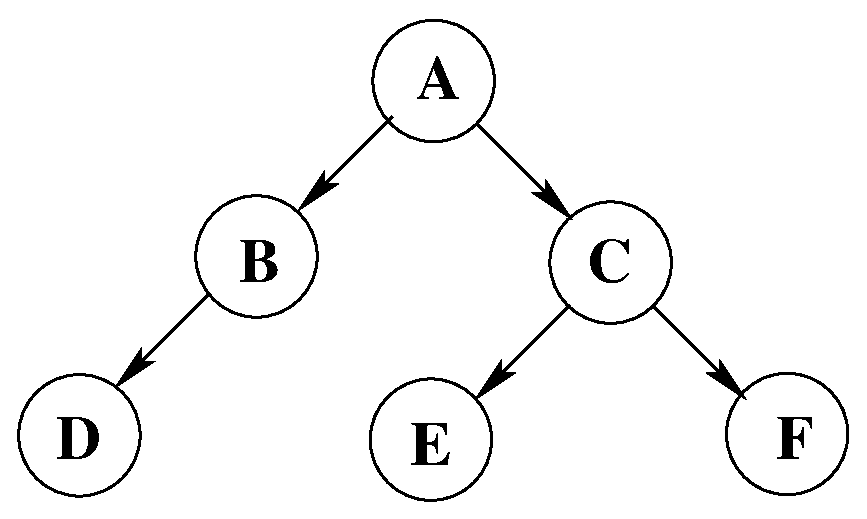
\includegraphics[height=1.5in]{ABCDEF.eps}
\end{tabular}

From the Bayes' net we have

$$P(A,B,C,D,+e,-f) = P(A) P(B|A) P(C|A) P(D|B) P(+e|C) P(-f|C)$$

The order in which to joint factors is arbitrary, and we wil use B, C, A resulting in the factors below.

\begin{eqnarray*}
f_1(A,B,D)         &=& P(B|A) P(D|B) \\[.1in]
f_2(A,C,+e,-f)     &=& P(C|A) P(+e|C) P(-f|C) \\[.1in]
f_3(A,B,C,D,+e,-f) &=& P(A) f_1(A,B,D) f_2(A,C,+e,-f) \\[.1in]
\end{eqnarray*}

We need this for factor 2.
$$P(C) = P(C | A) * P(A)$$
\begin{center}
\begin{tabular}{|c|c|c|c|c|} \hline
A & C & $P(C|A)$  &  P(A) & P(C) \\ \hline
+a & +c  & 0.2 & 0.3 & 0.06  \\ \hline
+a & -c  & 0.8 & 0.3 & 0.24 \\ \hline
-a & +c  & 0.9 & 0.7 & 0.63 \\ \hline
-a & -c  & 0.1 & 0.7 & 0.07 \\ \hline
\end{tabular}
\hspace{1in}
\begin{tabular}{|c|c|} \hline
C & P(C) \\ \hline
+c & 0.69 \\ \hline
-c & 0.31 \\ \hline
\end{tabular}
\end{center}

Fill in the following factor tables:

\begin{center}
\begin{tabular}{cc}
\begin{tabular}{|r|r|r|l|} \hline
A  & B  & D  & $f_1(A,B,D)$ \\ \hline
+a & +b & +d & 0.7 * 0.3 = 0.21 \\ \hline
+a & +b & -d & 0.7 * 0.7 = 0.49 \\ \hline
+a & -b & +d & 0.3 * 0.4 = 0.12 \\ \hline
+a & -b & -d & 0.3 * 0.6 = 0.18 \\ \hline
-a & +b & +d & 0.6 * 0.3 = 0.18 \\ \hline
-a & +b & -d & 0.6 * 0.7 = 0.42 \\ \hline
-a & -b & +d & 0.4 * 0.4 = 0.16 \\ \hline
-a & -b & -d & 0.4 * 0.6 = 0.24 \\ \hline
\end{tabular} &
\raisebox{.41in}{\begin{tabular}{|r|r|l|} \hline
A  & C  & $f_2(A,C,+e,-f)$ \\ \hline
+a & +c & 0.2 * (0.4 / 0.69) * (0.9 / 0.69) = 0.151 \\ \hline
+a & -c & 0.8 * (0.5 / 0.31) * (0.2 / 0.31) = 0.832 \\ \hline
-a & +c & 0.9 * (0.4 / 0.69) * (0.9 / 0.69) = 0.681 \\ \hline
-a & -c & 0.1 * (0.5 / 0.31) * (0.2 / 0.31) = 0.104 \\ \hline
\end{tabular}}
\end{tabular}


\end{center}

\vspace*{0.2in}

Using $f_1$ and $f_2$, compute $f_3$:

\begin{center}
\begin{tabular}{|r|r|r|r|l|} \hline
A  & B  & C  & D  & $f_3(A,B,C,D,+e,-f)$  \\ \hline
+a & +b & +c & +d & 0.3 * 0.21 * 0.151 = 0.0095\\ \hline
+a & +b & +c & -d & 0.3 * 0.49 * 0.151 = 0.0221\\ \hline
+a & +b & -c & +d & 0.3 * 0.21 * 0.832 = 0.0524\\ \hline
+a & +b & -c & -d & 0.3 * 0.49 * 0.832 = 0.1123\\ \hline
+a & -b & +c & +d & 0.3 * 0.12 * 0.151 = 0.0054\\ \hline
+a & -b & +c & -d & 0.3 * 0.18 * 0.151 = 0.0081\\ \hline
+a & -b & -c & +d & 0.3 * 0.12 * 0.832 = 0.0299\\ \hline
+a & -b & -c & -d & 0.3 * 0.18 * 0.832 = 0.0449\\ \hline
-a & +b & +c & +d & 0.7 * 0.18 * 0.681 = 0.0858\\ \hline
-a & +b & +c & -d & 0.7 * 0.42 * 0.681 = 0.2002\\ \hline
-a & +b & -c & +d & 0.7 * 0.18 * 0.104 = 0.0131\\ \hline
-a & +b & -c & -d & 0.7 * 0.42 * 0.104 = 0.0305\\ \hline
-a & -b & +c & +d & 0.7 * 0.16 * 0.681 = 0.0762\\ \hline
-a & -b & +c & -d & 0.7 * 0.24 * 0.681 = 0.1144\\ \hline
-a & -b & -c & +d & 0.7 * 0.16 * 0.104 = 0.0116\\ \hline
-a & -b & -c & -d & 0.7 * 0.24 * 0.104 = 0.0174\\ \hline
\end{tabular}
\end{center}
Then we marginalize over B,C, and D 
\begin{center}
\begin{tabular}{|r|l|} \hline
A  & $\sum_{B,C,D}f_3(A,B,C,D, +e,-f)$ \\ \hline
+a & 0.0095 + 0.0221 + 0.0524 + 0.1123 + 0.0054 + 0.0081 + 0.0299 + 0.0449 = 0.2846 \\ \hline
-a & 0.0858 + 0.2002 + 0.0131 + 0.0305 + 0.0762 + 0.1144 + 0.0116 + 0.0174 = 0.5492\\ \hline
\end{tabular}
\end{center}
Finally, we normalize to get our answer
\begin{center}
\begin{tabular}{|r|l|} \hline
A  & $P(A| +e,-f)$ \\ \hline
+a & 0.2846 / 0.8338 = 0.3413
 \\ \hline
-a & 0.5492 / 0.8338 = 0.6587\\ \hline
\end{tabular}
\end{center}

% 2015 hw07.

\end{document}
